\section{Aurdino and user interface setup}
\subsection{Arduino Setup}
The Arduino code runs the main functionality of the device. The glove reads in all the data from the sensors and filters out any inaccurate data points. It then sends that data to the GUI, before sorting each different kind of data point into an array and then calculating the average result. The averages are printed out on the LCD screen and then compared with the CDC reported temperature of 100.4 F / 38 C as well as the blood oxygen level of 96\%. If the patient’s temperature is above 100.4 or their blood oxygen level is below 96\% the glove will recommend further treatment which is printed out by the glove using the LCD screen. If neither result is abnormal then the glove reports the user as healthy and up to the physician’s discretion. The glove can function entirely on its own, but the companion program gives physicians much more data to work with. This data includes the patient’s blood oxygen level, temperature, heart rate, and the confidence level of the oximeter. We also added all of the code, pictures, and reports to a github repository with assembly instruction and documented code so that anyone can recreate our project.

\subsection{GUI Setup}
The GUI is written in Python, and it uses the serial communication to talk with Arduino. It shows show two graphs of the temperature and the blood oxygen of the patient, but the code can be maintainable and customizable to support heart rate too, or even ECG graphs.

The GUI is thoroughly written using an MVC pattern (Figure \ref{fig:MVC}), in order to let the application be actually extendible easily by anyone.

\begin{figure}[t]
    \centering
    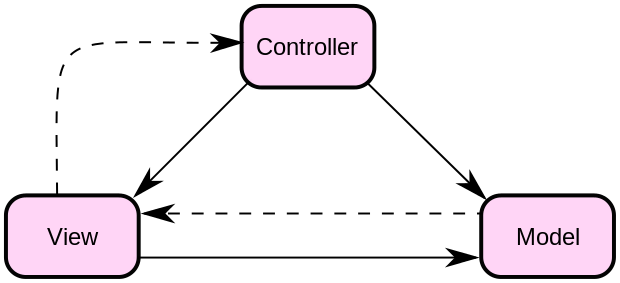
\includegraphics[width=\linewidth]{resources/MVC.png}
    \caption{MVC pattern}
    \label{fig:MVC}
\end{figure}

The application is a companion feature along with LCD: \textbf{it is not necessary}. The glove can be used without a laptop, or a device able to transmit a Python GUI. The device is been thought entirely to work without the GUI. In fact, this part of the application could be improved for further applications (Section \ref{sec:further})